\documentclass[a4paper,oneside,reqno]{amsart}
\usepackage{csvsimple}
\usepackage{longtable}

\input{../../../cambridge-macros.tex}

%    Set assignment information here
\newcommand{\authorname}{Feynman Liang}
\newcommand{\coursename}{MLSALT 9: Statistical Spoken Dialogue Systems}
\newcommand{\assignmentname}{Practical}

\begin{document}

%\includepdf[noautoscale]{MLSALT_Coversheet.pdf}

\title{\coursename\\\assignmentname}

\author{\authorname}
\date{\today}

\maketitle

\section{Introduction}

In a statistical spoken dialogue system, speech is processed by ASR and
semantic decoding to yield a distribution over dialogue acts (i.e.\
SLU, spoken language understanding). The SLU output is then processed by a
\textbf{dialogue management} module to yield dialogue actions, which are synthesized
into speech and output back to the user.

\begin{figure}[ht]
  \begin{center}
    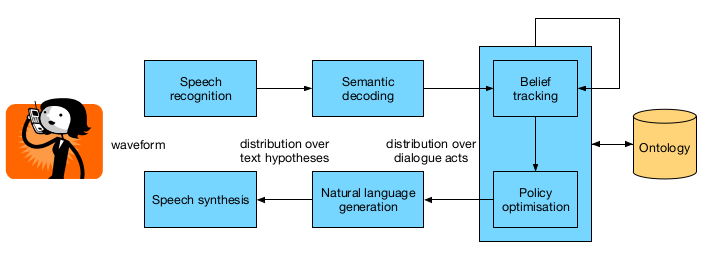
\includegraphics[scale=.5]{Figures/ds-diagram.png}
  \end{center}
  \caption{Schematic of a statistical spoken dialogue system\cite{lect3}}
  \label{fig:schematic}
\end{figure}

This practical investigates two dialogue management components: \textbf{belief
state tracking} and \textbf{policy optimization}. The belief state is a
representation of the user's intentions using SLU evidence accumulated from the
current and prior dialogue turns. The belief tracker updates the current belief
state given the prior belief state and current SLU output. In
\autoref{sec:focus}, we compare a baseline belief tracker solely utilizing the
most probable values from SLU against a focus tracker which combines prior
belief states with the SLU evidence.

The current belief state is used by the policy optimizer to yield dialogue
actions (i.e.\ responses for a dialogue turn). In this practical, we
investigate two reinforcement learning algorithms (Monte Carlo Control,
Gaussian process-SARSA) which both maintain an internal estimate of
$Q(\vec{b},a)$ representing the expected return of taking action $a$ in belief
state $\vec{b}$, i.e.
\begin{equation}
  \label{eq:Q}
  Q(\vec{b},a) = \ex\left\{ \sum_{k=0}^{T-t} \gamma^k r_{t+k} | b_t = b, a_t = a \right\}
\end{equation}
where $\gamma$ is the discount factor, $r_{t+k}$ is the reward at time $t+k$,
and the expectation is taken under the policy induced by $Q$ with $\epsilon$-greedy
action selection (i.e.\ on-policy).

\section{Dialogue state tracker}\label{sec:focus}

In this practical, we investigate discriminative methods for belief tracking
which model the condition distribution (i.e.\ $b(s_t) = p(s_t | o_t)$). One
advantage over generative models which model $b(s_t) = p(o_t|s_t) p(s_t)$ (see
\autoref{sec:conclusion}) is the ability to handle correlated input
features\cite{metallinou2013discriminative}.

A baseline method for state tracking consists of recording for each slot at
each turn the single hypothesis with the highest SLU score seen so far,
effectively performing an element-wise $\argmax$ (maximizing SLU scores) to
combine the prior belief state with the current SLU output. This assumes SLU
evidence from previous turns is just as important as the current SLU evidence,
ignoring the temporal dynamics of a dialogue episode and making it difficult to
handle global constraint changes.

In contrast, the focus tracker models the current belief as a convex combination
of the prior belief state and current SLU evidence:
\begin{align}
  q_{c,t} &= 1 - \sum_{v \in V_c} slu_{t,c}(v) \label{eq:q}\\
  p_{c,t}(v) &= \text{normalize}(slu_{t,c}(v) + q_{c,t} p_{c,t-1}(v)) \label{eq:pt}\\
  p_{c,1}(v) &= \text{normalize}(slu_{1,c}(v)) \label{eq:p0}
\end{align}
$q_{c,t}$ is the probability the SLU did not find any evidence about slot $c$
in turn $t$. If the current SLU provides more evidence for a slot $c$,
$q_{c,t}$ will be small hence the current belief (\autoref{eq:pt})
will be largely comprised of the SLU output. This model for belief state
dynamics gives more weight (``focus'') to slots which have lots of SLU evidence
and backs off to the prior belief state when there is
less SLU evidence (i.e.\ large $q_{c,t}$).

\subsection{Focus tracker implementation}

In \autoref{lst:focus-goal} we implement the focus tracker's
belief state update rule (\autoref{eq:pt}) for goal tracking.

\lstinputlisting[firstnumber=339,firstline=339,lastline=344,caption=Focus goal
tracking,label=lst:focus-goal]{
cued-python_practical/practical1_dst/scripts/baseline.py}

In \autoref{lst:focus-method} we implement \autoref{eq:pt} for method tracking.
Unlike goal tracking, which maintains a belief distribution over values for
each slot and hence runs inside of a \texttt{for} loop over \texttt{slot}s),
there is only a single distribution over all possible methods.

\lstinputlisting[firstnumber=355,firstline=355,lastline=359,caption=Focus method
tracking,label=lst:focus-method]{
cued-python_practical/practical1_dst/scripts/baseline.py}

\autoref{lst:focus-req} implements focus requested slot tracking. Since a slot
is no longer requested after it has been informed, we set the score of all
slots appearing in \texttt{informed\_slots} to be zero. For slots not appearing in
\texttt{informed\_slots}, we combine the SLU evidence with the previous belief
according to \autoref{eq:pt}.

\lstinputlisting[firstnumber=377,firstline=377,lastline=385,caption=Requested
slot tracking,label=lst:focus-req]{
cued-python_practical/practical1_dst/scripts/baseline.py}

\subsection{Performance comparison}

We evaluate the performance of the baseline (\autoref{tab:baseline-tracker})
and focus (\autoref{tab:focus-tracker}) tracker on the DSTC \textbf{dtsc2\_data}
dataset.

\begin{table}[ht!]
  \begin{tabular}{cccc}
    \toprule
                  &   Joint Goals   &    Requested    &      Method    \\
    \midrule
    Accuracy      &    0.5686546    &    0.9162437    &    0.8529820   \\
    l2            &    0.8344502    &    0.1204444    &    0.2560611   \\
    roc.v2\_ca05  &    0.0000000    &    0.6066482    &    0.0016260   \\
    \bottomrule
  \end{tabular}
  \caption{Baseline tracker performance}
  \label{tab:baseline-tracker}
\end{table}

\begin{table}[ht!]
  \begin{tabular}{cccc}
    \toprule
                  &   Joint Goals   &    Requested    &      Method    \\
    \midrule
    Accuracy      &    0.7323162    &    0.9162437    &    0.5492372   \\
    l2            &    0.4212595    &    0.1194034    &    0.7911165   \\
    roc.v2\_ca05  &    0.0000000    &    0.5623269    &    0.0000000   \\
    \bottomrule
  \end{tabular}
  \caption{Focus tracker performance}
  \label{tab:focus-tracker}
\end{table}

The focus tracker has improved across all metrics for goals tracking. This
suggests that the focus tracker better models the belief state dynamics,
possibly because it can allow the SLU output to override the previous belief
state and hence handle changing goal constraints. The requested slot tracking
performance is similar, with identical accuracies and negligible difference in
l2 values.

However, focus method tracking performance is below baseline. This suggests that
method does not usually change during a dialogue episode and hence keeping the
1-best semantic decoding prediction suffices.

\section{Monte Carlo control algorithm}

We view dialogue policy optimization as a reinforcement learning problem, where
the dialogue act must be selected given the current belief state to maximize
some measure of dialogue quality.  Monte Carlo control (MCC) is a model-free
algorithm for the reinforcement learning problem. It learns a $Q$-function
(\autoref{eq:Q}) by averaging sample returns over complete episode.

In our implementation, the $Q$-function is represented by a dictionary $\cd$
containing $Q(\vec{b},a)$ for a grid of $(\vec{b},a)$ reference points. Since there are
uncountably many $\vec{b} \in \RR^n$, sparsification and nearest neighbor
interpolation is used to limit the size of the dictionary. We only add a
$(\vec{b},a)$ point to the dictionary if
\[
  \forall (\vec{b}',a') \in \cd: \|(\vec{b},a) - (\vec{b}',a')\| > \nu
\]
Otherwise, the nearest neighbor
\[
  (\vec{b}^*,a^*) = \argmin_{(\vec{b}',a') \in \cd} \|(\vec{b},a) - (\vec{b}',a')\|
\]
is used for updating the $Q$-function estimate and evaluating $Q(\vec{b},a)$.

As a result of nearest neighbor interpolation, MCC approximates $Q$ with
step functions over the Voronoi partitions defined by $(\vec{b},a) \in \cd$.
These sharp discontinuities in $Q$ may be unrealistic.

To trade off exploration and exploitation, $\epsilon$-greedy action
selection is used for episode generation. This directs the MCC algorithm
to exploit the current estimate and greedily select the action maximizing $Q$
with probability $1 - \epsilon$ and to explore a random action with probability
$\epsilon$.

\subsection{Performance of MCC policy}

\autoref{fig:mcc} shows the average success per iteration for MCC policy using
a focus belief tracker with the simulated user under concept error rate
$r=15\%$.

\begin{figure}[ht!]
  \begin{center}
    \includegraphics[scale=1.0]{Figures/mcc.pdf}
  \end{center}
  \caption{MCC success per dialogue turn, error bars $\pm$ 1 stdev}
  \label{fig:mcc}
\end{figure}

Notice that performance deteriorates when the sparsification threshold $\nu$ is
large (e.g. $\geq 0.05$). This is likely due to over-sparsification: setting
$\nu$ too large results in few $(\vec{b},a)$ grid points in $\cd$ and an
over-smoothed estimate for $Q$.

Lower $\nu$ values achieve greater success, but at the cost of increasing the
number of grid points used in estimating $Q$. This increases the memory
required to store the $Q$-function estimate as well as the computational
complexity of evaluating $Q$ for a new point.

Another consideration for choosing $\nu$ is its effect as a regularizer.  As
step functions over a sparse grid is a more restrictive model class than a
dense grid, $\nu$ may also be interpreted as a form of regularization
decreasing the variance of the $Q$-function estimator. Setting $\nu$ too low
may result in overfitting and worse generalization.

\section{Episodic GP-SARSA policy}\label{sec:gp}

Estimating $Q$ using a Gaussian process instead of nearest-neighbor
interpolation motivates GP-SARSA, a non-parametric approach to policy
optimization. Instead of modeling $Q$ using step functions on a Voronoi
partition, GP-SARSA\cite{engel2005reinforcement} places a Gaussian Process
prior over $Q$, i.e.
\[
  Q(\vec{b},a) \sim \cg\cp(0, k((\vec{b},a),(\vec{b},a)))
\]
and use the MAP of the predictive posterior for estimating $Q(\vec{b},a)$.
Knowledge (through $k(\cdot,\cdot)$) about similarity in the observation space
enables explicit modeling of smoothness assumptions and increases policy
learning speed.

We investigate linear
\begin{equation}
  \label{eq:linear}
  k((\vec{b},a),(\vec{b}',a')) = \langle \vec{b}, \vec{b}'\rangle \delta_a(a')
\end{equation}
and Gaussian
\begin{equation}
  \label{eq:gaussian}
  k((\vec{b},a),(\vec{b}',a')) = p^2 \exp\left( -\frac{\|\vec{b} - \vec{b}'\|^2}{2l^2} \right) \delta_a(a')
\end{equation}
covariance kernels. Both kernels include $\delta_a(a')$, removing any
covariance between $(\vec{b},a)$ pairs from different actions.


The linear kernel assumes that covariances are generated from inner products.
It accounts for collinearity and will always yield $0$ for orthogonal beliefs
$\vec{b}$ and $\vec{b}'$ regardless of how small $\|\vec{b} - \vec{b}'\|$ may
be.  It is unclear that an inner product, which is bilinear by definition, is a
good way to measure similarity. In particular, bilinearity requires antipodal
belief states to be negatively correlated. If $Q$ is non-linear (e.g.
$Q(\vec{b},a) = \|\vec{b}\|$), this restriction may be unrealistic.

In contrast, a Gaussian kernel's value is directly related $\|\vec{b} -
\vec{b}'\|$.  The Gaussian kernel can be interpreted as placing Gaussians
centered at each of the dictionary points. It makes the weaker modeling
assumption that points closer in $\ell_2$ distance should have higher
covariance. Unlike linear kernels which assume $Q$ to be linear, Gaussian
kernels only assume that $Q$ varies smoothly on some characteristic length
scale $l$ with noise variance $p$.

Computing the Gram matrix $\tilde{\matr{K}}$ ($\in O(N^3)$) is required for
computing the predictive posterior and estimating $Q$ at new locations. To
limit computational complexity, sparsification is used to approximate the
$\tilde{\matr{K}}$ with a dictionary of representative points $\cd$. A point
$(\vec{b}^t, a^t)$ is added to $\cd$ only if the approximate linear dependence
(ALD) condition holds:
\begin{equation}
  \label{eq:ald}
  \min_{\vec{g}_t \in \\R^{|\cd|}}
  \left\|
  \sum_{(\tilde{b}^j,\tilde{a}^j) \in \cd} \vec{g}_{t,j} \phi(\tilde{b}^j, \tilde{a}^j) - \phi(\vec{b}^t, a^t)
  \right\|^2
  \geq \nu
\end{equation}

\autoref{eq:ald} makes sense because kernel functions are used in the ``kernel trick''
to efficiently evaluate high dimensional inner products, i.e.
\[
  k((\vec{b},a),(\vec{b}',a')) = \langle \phi(\vec{b},a), \phi(\vec{b}',a') \rangle
\]
where $\phi(\vec{b},a)$ is a (possibly high-dimensional) feature vector. If
\autoref{eq:ald} fails to hold, then
\[
  \phi(\vec{b}^t, a^t) \approx \sum_{j=0}^m \vec{g}_{t,j} \phi(\tilde{b}^j, \tilde{a}^j)
\]
hence by bilinearity of inner product
\begin{align}
  k((\vec{b}^t, a^t), (\vec{b}', a')) \nonumber
  &= \langle \phi(\vec{b}^t, a^t), \phi(\vec{b}', a') \rangle \nonumber\\
  &\approx \langle \sum_{j=0}^m \vec{g}_{t,j} \phi(\tilde{b}^j, \tilde{a}^j), \phi(\vec{b}', a') \rangle \nonumber\\
  &= \sum_{j=0}^m \vec{g}_{t,j} \langle \phi(\tilde{b}^j, \tilde{a}^j), \phi(\vec{b}', a') \rangle \nonumber\\
  &= \sum_{j=0}^m \vec{g}_{t,j} k((\tilde{b}^j, \tilde{a}^j), (\vec{b}', a')) \nonumber
\end{align}
so the kernel function $k((\vec{b}^t, a^t), \cdot)$ can be approximated by the
kernel function $k((\tilde{b}^j, \tilde{a}^j), \cdot)$ at existing dictionary
points $(\tilde{b}^j, \tilde{a}^j) \in \cd$ hence $(\vec{b}^t, a^t)$ is not added
to $\cd$.

The left hand side of \autoref{eq:ald} is equal to the squared norm of the
orthogonal projection and will be equal to $0$ if $(\vec{b}^t, a^t)$ is in the
kernel span (column span of $\tilde{\matr{K}}$). In particular, this implies
that the dictionary will be linearly independent and hence contain at most
$\dim \text{Range}(\varphi)$ entries.  For linear kernels,
$\phi(\vec{b}^t, a^t) = \vec{b}^t$ so we can upper bound
\[
  |\cd| \leq \dim \phi(\vec{b},a) = \dim \vec{b}
\]
This is less useful for Gaussian kernels, where the feature space corresponding
to the Gaussian kernel RKHS is (countably) infinite dimensional.

\subsection{Performance of GP-SARSA}

\autoref{fig:gp} compares the best MCC policy ($\nu=0.01$) against GP-SARSA
with various kernels using a focus belief tracker on the simulated user under
concept error rate $r=15\%$.

\begin{figure}[ht!]
  \begin{center}
    \includegraphics[scale=1.0]{Figures/gp.pdf}
  \end{center}
  \caption{GP-SARSA success per dialogue turn, error bars $\pm$ 1 stdev}
  \label{fig:gp}
\end{figure}

Almost all GP-SARSA settings achieved better performance than the MCC policy.
This suggests that the smoothness assumptions of the GP prior is a better fit
for the true $Q$-function than the piecewise constant model used in MCC's
nearest-neighbor interpolation.

The performance of Gaussian kernels can exceed the performance of the linear
kernel, but is sensitive to the parameters $p$ and $l$. We tried a grid of
parameters with $p \in \{2,3,4,5\}$ and $l \in \{2,3,4\}$ and report the linear
kernel and top two Gaussian kernel results in \autoref{fig:gp}.
\autoref{fig:gp} shows that a Gaussian kernel with length scale $l=2$ and noise
variance $p=4$ yields consistently good performance within the $70-80\%$
success range.

\section{Conclusion}\label{sec:conclusion}

This practical investigated two belief trackers and two policy optimizers. We
found focus tracking to yield better goal tracking but worse method tracking
compared to the baseline tracker. In policy optimization, we found GP-SARSA
offered significant performance gains over MCC and identified a Gaussian kernel
with variance $p=3$ and length scale $l=2$ yielded consistently good
performance.

\subsection{Connections to lecture}

In generative belief tracking, the belief state $b(s_t)$ models the joint
probability $p(o_t|s_t)p(s_t)$ and dialogue management is treated as a POMDP
While POMDPs are mostly intractable, approximations for specific cases are
available. Hidden Information State\cite{young2010hidden}
factorizes the dialogue state into user acts, user goals, and dialogue
histories and uses hand-crafted transitions, grouping of goals, and pruning to
achieve tractability. Bayesian Update of Dialogue
States\cite{thomson2010bayesian} further factorizes the belief state to permit
tractable belief tracking as well as variational estimation of the transition
$p(s_{t+1}|s_t,a_t)$ and emission $p(o_t|s_t)$ probability distributions using
expectation propagation.

In class-based belief tracking, classifiers such as decision
trees\cite{williams2014web} or deep neural networks
windows\cite{henderson2014word} are used to predict state posterior
probabilities given the observation history. Recurrent neural networks can be
used for potentially infinite context length\cite{henderson2015discriminative}.
Also, it is possible to directly map from ASR hypotheses to belief states,
avoiding the semantic decoder entirely\cite{henderson2014word}. \cite{lect4}
shows that both decision trees and RNNs outperform the focus tracker. It also
shows RNNs trained directly on ASR outputs achieved higher accuracy and ROC
than those trained on semantic decoding outputs. Doing this, however, requires
us to have access to the hypotheses generated by the ASR system.

In policy optimization, we could have considered temporal-difference methods
such as natural actor critic\cite{thomson2013statistical}. Use of a critic
reduces variance, resulting in more stable learning, and the natural
gradient\cite{amari1998natural} speeds up convergence.  However, computing the
natural gradient requires a parametric and differentiable estimator for $Q$, hence
it is incompatible with both MCC and GP-SARSA.

\subsection{Extensions}

One possible extension is to utilize an ensemble of models for class-based
belief tracking. This allows combination of multiple classification models
(e.g. RNNs, Random Forests) trained on different data sources (e.g. ASR,
multiple semantic decoders).

Another extension is to use a different metric when measuring the
distance between two belief vectors (e.g. \autoref{eq:gaussian}). Since belief
states $\vec{b}$ are formed by concatenating normalized probability vectors,
they are highly constrained and exist on a sub-manifold. Instead of $\ell_2$
norm, a more appropriate metric such as geodesic distance on the sub-manifold
could be used.

Finally, SARSA is on-policy and updates $Q$ according to the actual subsequent
state-action $(s',a')$ pair. Instead, a possible extension could be to
investigate off-policy methods like $Q$-learning (which replaces $Q(s',a')$
with $\argmax_a Q(s',a)$).  Since off-policy methods do not account for
$\epsilon$-greedy action selection, we would expect them to perform worse
during training but better during exploitation (i.e.\ no $\epsilon$-greedy
exploration).


\bibliographystyle{alpha}
\nocite{*}
\bibliography{refs}

%\appendix

%\section{Experimental Result Data Tables}

%\csvreader[longtable=llll,
  %table head={%
    %\caption{All results for MCC policy}\label{tab:mcc} \\
    %\toprule Nu & Iteration & Success.Mean & Success.Std\\\midrule
  %},
  %table foot=\bottomrule]%
%{mcc-data.csv}{1=\nu,2=\iter,5=\mean,6=\std}%
%{\nu & \iter & \mean & \std }%

%\csvreader[longtable=llll,
  %table head={%
    %\caption{All results for GP-SARSA policy}\label{tab:gp} \\
    %\toprule Kernel & Iteration & Success.Mean & Success.Std\\\midrule
  %},
  %table foot=\bottomrule]%
%{results-all-tidy-report.csv}{1=\kernel,2=\iter,3=\mean,4=\std}%
%{\kernel & \iter & \mean & \std }%

\end{document}
